\documentclass[a4paper]{article}

\author{Буренин А.А}


% Packages
\usepackage{amsmath}
\usepackage[14pt]{extsizes}

\usepackage{fontspec}
\setromanfont{Times New Roman}

\usepackage[utf8]{inputenc}
\usepackage[russian]{babel}
\usepackage{multicol}
\usepackage[
    a4paper,
    left=30mm,
    right=15mm,
    top=20mm,
    bottom=20mm,
    nohead,
    footskip=10mm
]{geometry}
\usepackage{graphicx}
\usepackage{textcomp}
\usepackage{tocloft}
\usepackage{titlesec}
\usepackage{ragged2e}
\usepackage{hyperref}
\usepackage{textcase}
\usepackage{sectsty}
\usepackage{sidecap}


\graphicspath{{./imgs/}}

% Подключает команду \mireatile
\newcommand{\mireatitle}[5]{{
    \clearpage
    \begin{center}
        
\includegraphics[width=30mm]{../static/logo}

        \footnotesize{МИНИСТЕРСТВО НАУКИ И ВЫСШЕГО ОБРАЗОВАНИЯ РОССИЙСКОЙ ФЕДЕРАЦИИ}

        \small
        Федеральное государственное бюджетное образовательное учреждение высшего образования

        \textbf{<<МИРЭА Российский технологический университет>>}

        \vspace{1.5em}

        \textbf{\large{РТУ МИРЭА}}
        \vspace{1.5em}

        \hline \hline

        \vspace{1.5em}

        \normalsize

        Институт информационных технологий

        Кафедра общей информатики

        \vspace{3em}

        \textbf{ОТЧЕТ}

        \textbf{ПО ПРАКТИЧЕСКОЙ РАБОТЕ № #1}

        \textbf{по дисциплине}

        <<ИНФОРМАТИКА>>


    \end{center}
    \vspace{6em}
    Выполнил студент группы #2 \hfill #3

    \vspace{1.7em}

    \flushleft{Принял \hfill #4}

    \textit{#5}

    \vspace{2em}


        \begin{tabular}{lrr}
            Практическая работа &
            <<\makebox[20pt][l]{\hrulefill}>>\makebox[80pt][r]{\hrulefill} 2022 г. &
            \makebox[30pt][k]{\hfill} \\

            выполнена \\

            <<Зачтено>> &
            <<\makebox[20pt][l]{\hrulefill}>>\makebox[80pt][r]{\hrulefill} 2022 г. &
            \makebox[30pt][k]{\hfill} \\

            \vspace*{\fill} % Заполняет пространство по вертикали
        \end{tabular}

    \begin{center}
        Москва, 2022
    \end{center}
    \thispagestyle{empty} % Убирает номер страницы
    \clearpage
}}


% Каким-то макаром делает загаловки в содержании
% написанными большими буквами
\makeatletter
\let\oldcontentsline\contentsline
\def\contentsline#1#2{%
    \expandafter\ifx\csname l@#1\endcsname\l@section
    \expandafter\@firstoftwo
    \else
    \expandafter\@secondoftwo
    \fi
    {%
        \oldcontentsline{#1}{\MakeTextUppercase{#2}}%
    }{%
        \oldcontentsline{#1}{#2}%
    }%
}
\makeatother


% Центрирует заголовок содержания
\renewcommand\cfttoctitlefont{\hfill\Large\bfseries\MakeUppercase}
\renewcommand\cftaftertoctitle{\hfill\mbox{}}

% Убирает полужирность у элементов содержания
\renewcommand\cftsecfont{\mdseries}

% Центрирует заголовки секций
\titleformat{\section}[block]{\large\bfseries\filcenter}{}{1em}{}
\sectionfont{\large\bfseries\centering\MakeUppercase}

% Команды для секций
\newcommand{\introduction}{\section{Постановка задачи}\label{sec:introduction}}
\newcommand{\implementation}{\section{Проектирование и реализация}\label{sec:implementation}}
\newcommand{\conclusion}{\clearpage\section{Выводы}\label{sec:conclusion}}
\newcommand{\sources}{\clearpage\section{Информационные источники}\label{sec:sources}}



\begin{document}

    % номер практики, номер группы, имя студента, имя преподавателя, должность преподавателя
    \mireatitle{5}{ИКБО-14-22}{Буренин А.А.}{Павлова Е. С.}{ассистент}

    \tableofcontents{}

    \clearpage


    \introduction
    Логическая функция от четырех переменных задана в 16-ичной векторной форме.
    Восстановить таблицу истинности.
    Записать формулы СДНФ и СКНФ.
    Построить комбинационные схемы СДНФ и СКНФ в лабораторном комплексе,
    используя общий логический базис.
    Протестировать работу схем и убедиться в их правильности.
    Подготовить отчет о проделанной работе и защитить её.

    Логическая функция из персонального варианта:
    \[ F(a, b, c, d) = 6c6f_{16} \]


    \implementation

    \subsection{Восстановление таблицы истинности}\label{subsec:table-recovering}
    Преобразовав шестнадцатеричный вектор в двоичную СС, получаем восстановленную таблицу
    истинности для $ F $ (Таблица~\ref{tab:truth}).

    \begin{table}[h]
        \begin{center}
            \begin{tabular}{ | c | c | c | c | c | }
                \hline
                $ a $ & $ b $ & $ c $ & $ d $ & $ F $ \\
                \hline
                0     & 0     & 0     & 0     & 0     \\
                \hline
                0     & 0     & 0     & 1     & 1     \\
                \hline
                0     & 0     & 1     & 0     & 0     \\
                \hline
                0     & 0     & 1     & 1     & 1     \\
                \hline
                0     & 1     & 0     & 0     & 1     \\
                \hline
                0     & 1     & 0     & 1     & 0     \\
                \hline
                0     & 1     & 1     & 0     & 1     \\
                \hline
                0     & 1     & 1     & 1     & 0     \\
                \hline
                1     & 0     & 0     & 0     & 0     \\
                \hline
                1     & 0     & 0     & 1     & 1     \\
                \hline
                1     & 0     & 1     & 0     & 1     \\
                \hline
                1     & 0     & 1     & 1     & 1     \\
                \hline
                1     & 1     & 0     & 0     & 0     \\
                \hline
                1     & 1     & 0     & 1     & 1     \\
                \hline
                1     & 1     & 1     & 0     & 1     \\
                \hline
                1     & 1     & 1     & 1     & 1     \\
                \hline
            \end{tabular}
        \end{center}
        \caption{Таблица истинности}
        \label{tab:truth}
    \end{table}

    \subsection{Формулы СКНФ и СДНФ}\label{subsec:formulas}
    По восстановленной таблице истинности (Таблица~\ref{tab:truth}) запишем формулы СДНФ и СКНФ.
    Для построения формулы СДНФ рассматриваем наборы значений переменных, на которых функция равна единице.
    Переменные, равные нулю, берем с отрицанием, а переменные, равные единице, без отрицания.
    В результате этого мы получаем несколько совершенных конъюнкций, объединенных через дизъюнкцию.
    Это образует формулу СДНФ~\eqref{eq:sdnf}.

    \begin{equation}
        \label{eq:sdnf}
        F_{СДНФ}=\bar a \bar b \bar c d + \bar a \bar b c \bar d + \bar a b \bar c \bar d + \bar a b \bar c d + a \bar b \bar c d + a \bar b c \bar d + ab \bar c \bar d + ab \bar c d + abc \bar d + abcd
    \end{equation}

    Для построения формулы СКНФ рассматриваем наборы значений переменных, на которых функция равна нулю.
    Переменные, равные нулю, берем без отрицания, а переменные, равные единице, с отрицанием.
    В результате чего мы получаем несколько совершенных дизъюнкций, объединенных через конъюнкцию.
    Это образует формулу СКНФ~\eqref{eq:sknf}.


    \begin{equation}
        \label{eq:sknf}
        F_{СКНФ}=(a + b + c + d)\cdot(a + b + \bar c + \bar d)\cdot(a + \bar b + \bar c + d)\cdot(\bar a + b + c + d)\cdot(\bar a + b + \bar c + \bar d)
    \end{equation}

    \subsection{Схемы, реализующие СДНФ и СКНФ в общем логическом базисе}\label{subsec:schemas}
    Построим в лабораторном комплексе комбинационные схемы, реализующие СДНФ (Рисунок~\ref{fig:sdnf}) и СКНФ (Рисунок~\ref{fig:sknf}) рассматриваемой функции в общем логическом базисе.

    \begin{figure}[h]

        \centering
        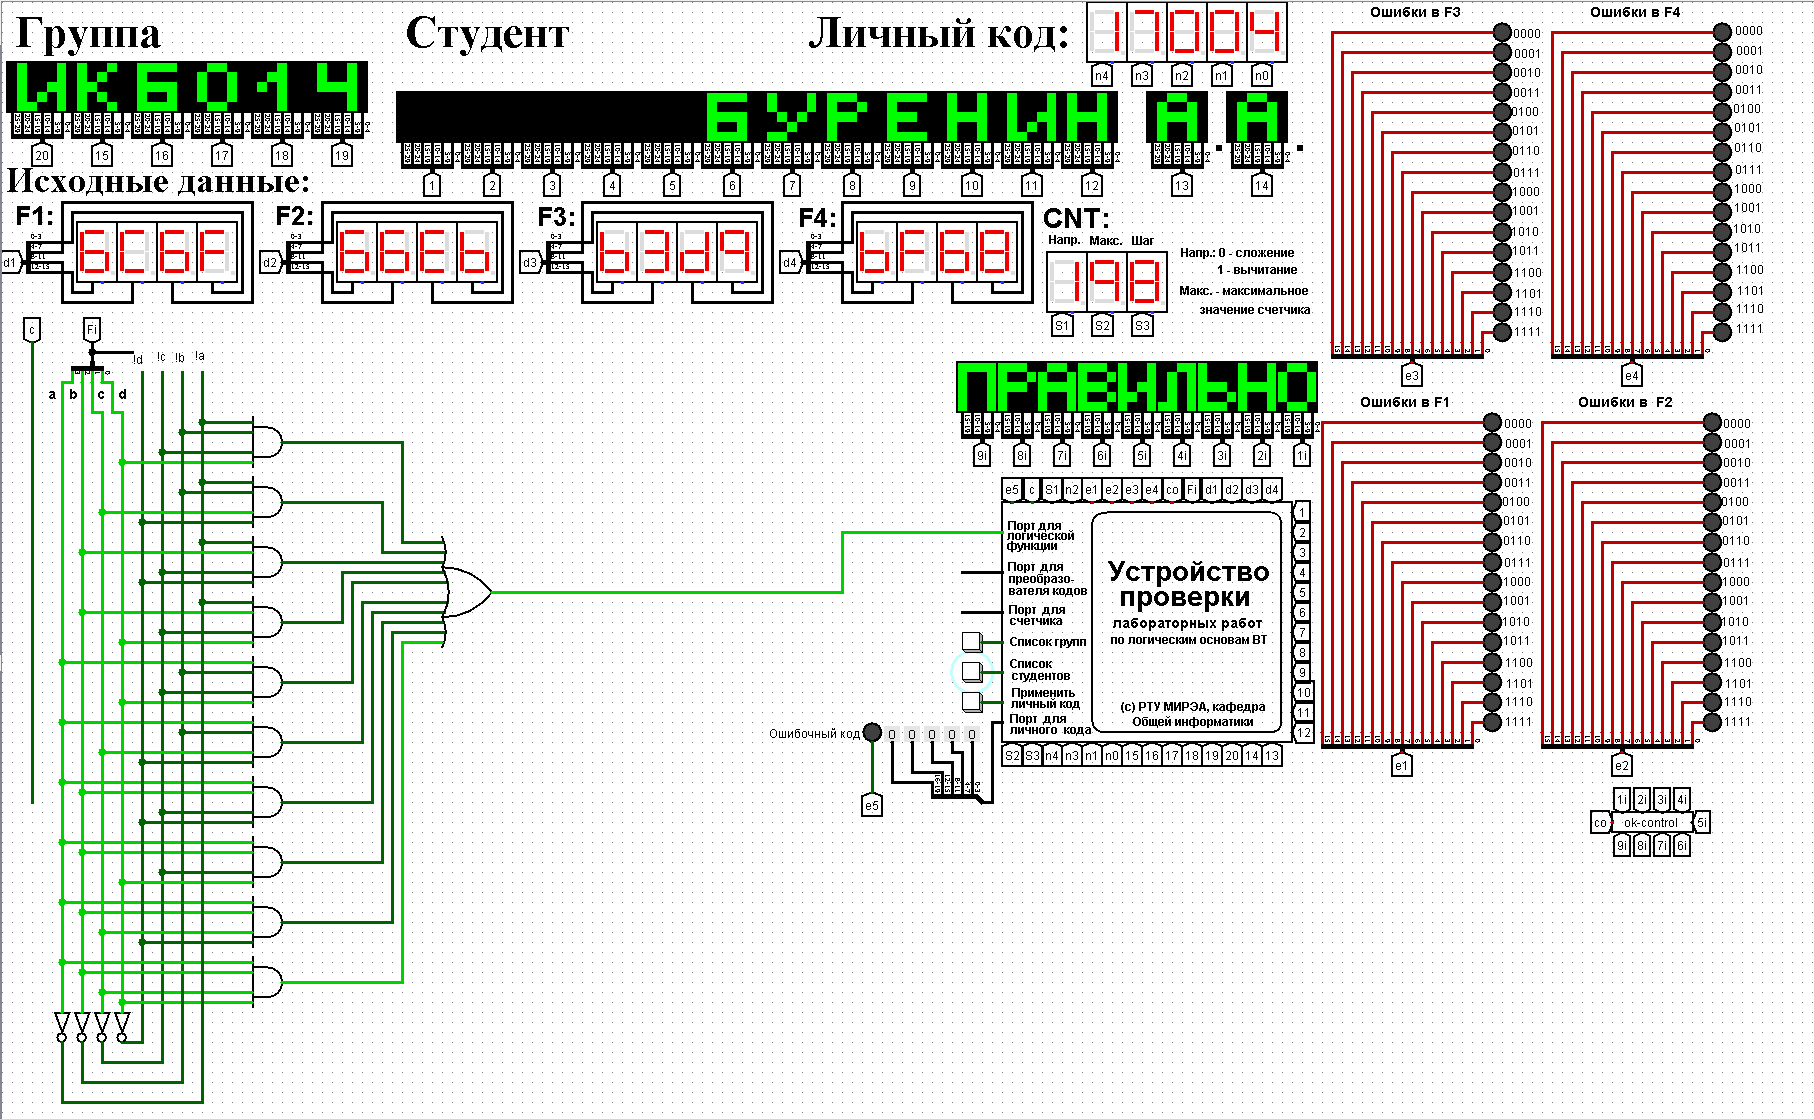
\includegraphics[width=0.8\textwidth]{sdnf.png}

        \caption{\centering Комбинационная схема, реализующая СДНФ в общем логическом базисе.}
        \label{fig:sdnf}
    \end{figure}

    \begin{figure}[h]
        \centering
        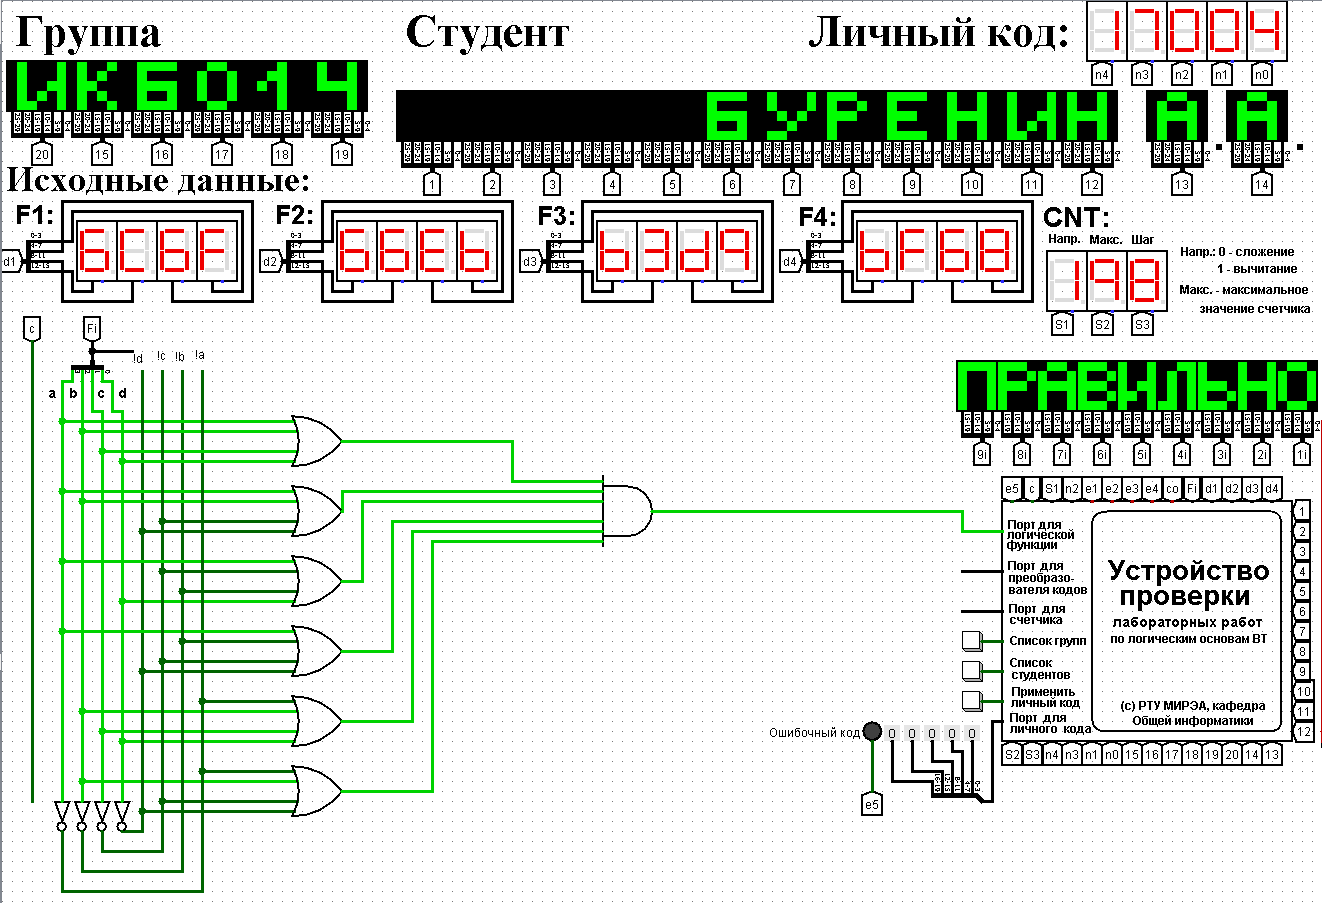
\includegraphics[width=0.8\textwidth]{sknf.png}

        \caption{\centering Комбинационная схема, реализующая СКНФ в общем логическом базисе.}
        \label{fig:sknf}
    \end{figure}


    \conclusion
    По данной логической функции от четырех переменных, заданной в шестнадцатеричной векторной форме
    была восстановлена таблица истинности (Таблица~\ref{tab:truth}).
    По ней были составлены формулы СДНФ~\eqref{eq:sdnf} и СКНФ~\eqref{eq:sknf}.
    Построены комбинационные схемы СДНФ (Рисунок~\ref{fig:sdnf}) и СКНФ (\ref{fig:sknf})
    в лабораторном комплексе с использованием общего логического базиса.
    Протестирована работа схем и их правильность.


    \sources
    \begin{enumerate}
        \item Информатика: Методические указания по выполнению практических
        работ / С.С. Смирнов, Д.А. Карпов - М., МИРЭА - Российский технологический университет, 2020.–102 с.
        \item Лекционный материал / С.С. Смирнов.
    \end{enumerate}

\end{document}
